\section{Methodology}
This section aims to describe the proposed approach to transform aggregated quantities of heat generation per technology to local heat network infrastructure topologies. The presented approach can be seen as a novel downscaling technique and is made, in particular, by two sequencing algorithms. Thereby, tailor-made indicators play a crucial role and serve as termination criteria for the downscaling process. Figure \ref{fig:meth1} illustrates the proposed idea to obtain local heat network topologies from IAM results. Thereby, \textit{Algorithm1} transforms heat generation per technology from the region level (e.g., country) to the sub-region level (e.g., NUTS3) taking into account empirical settings for network infrastructure requirements of heat technologies on the sub-region level. Afterwards, \textit{Algorithm2} disaggregates the results from the sub-region level to the small sub-region level (LAU) to obtain local heat networks and improve their network topology. The iterative application of the latter algorithm enables an improvement of the network topology by each iteration using a benchmarking with tailor-made indicators and leads to the local heat network topologies.\vspace{0.3cm}

\begin{figure}[h]
	\centering
	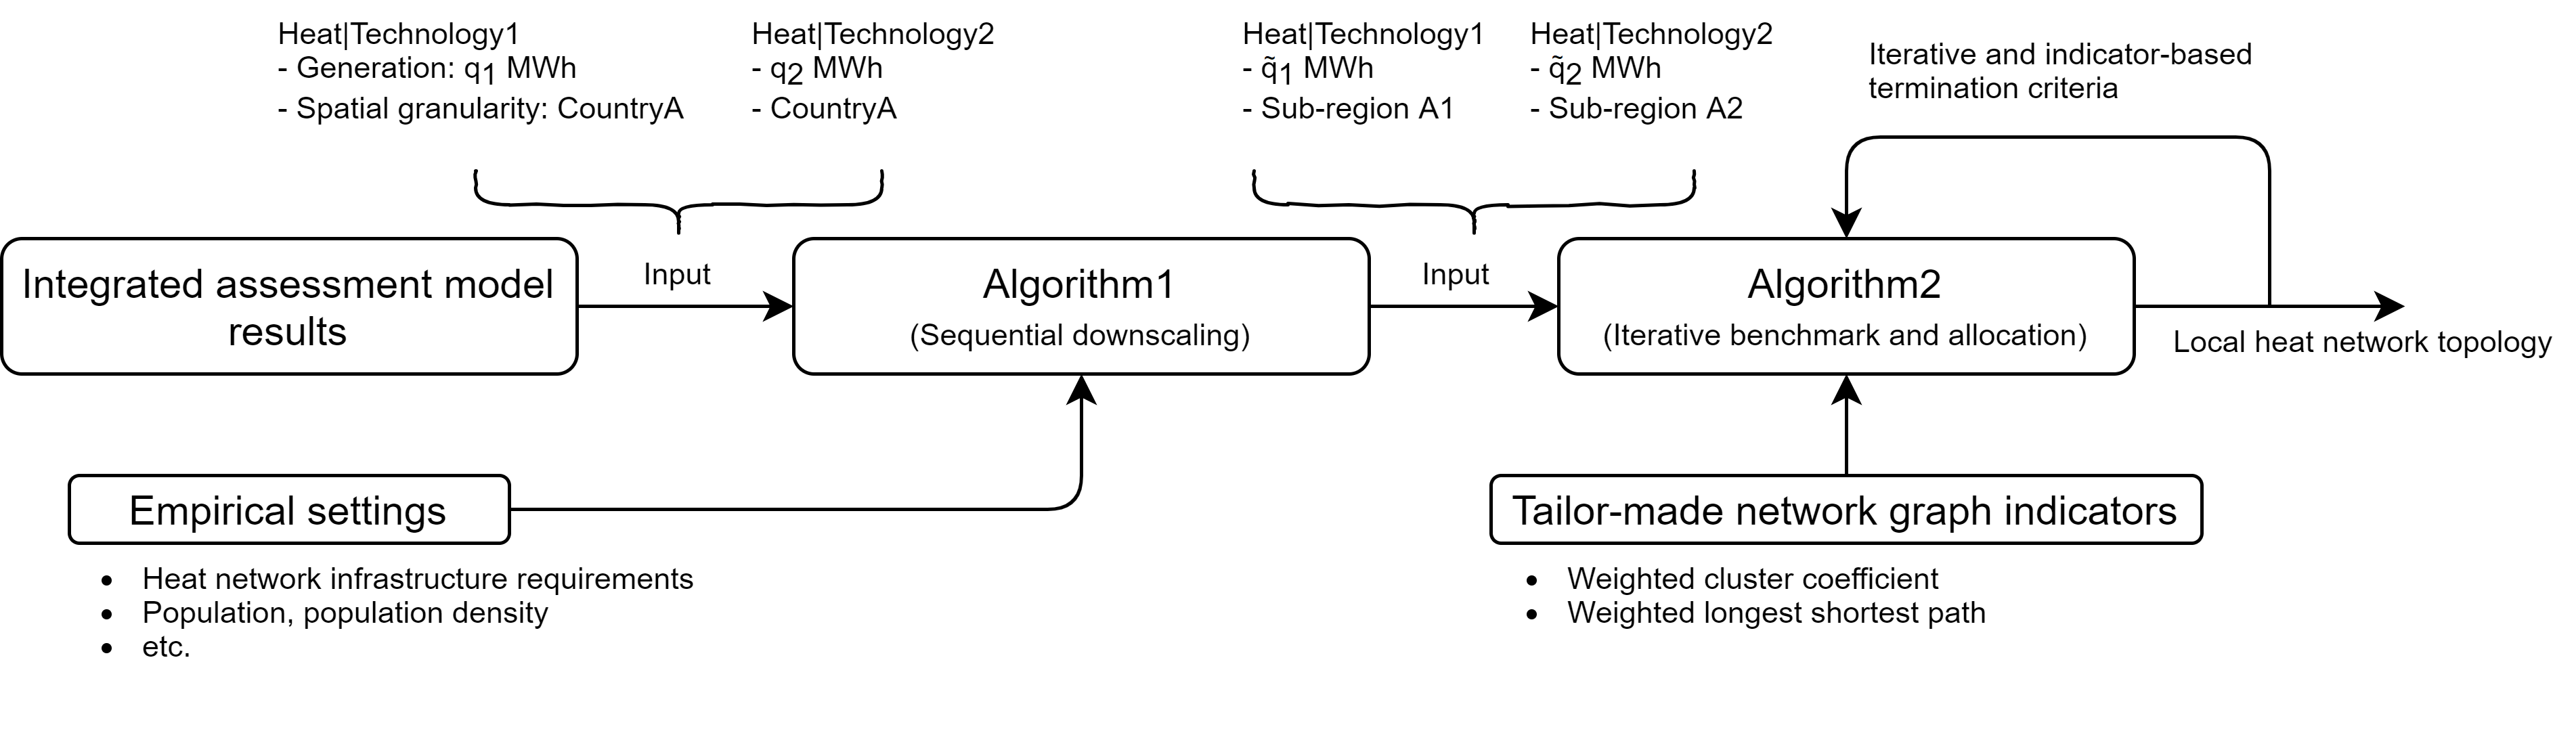
\includegraphics[width=1\linewidth]{figures/3_Methodology/Flow_diagram.png}
	\caption{Basic concept of the downscaling technique using two sequencing algorithms}
	\label{fig:meth1}
\end{figure}

\subsection{Algorithm1: Sequential downscaling disaggregating heat generation per technology from the region to the sub-region level}
Here, we describe the technique to downscale IAM results of the low temperature residential and commercial heating sector from the region (NUTS0) to the sub-region (NUTS3) level.\footnote{In principle, different tuples of spatial granularity between the spatial level of values to be downscaled and the desired spatial level of disaggregation could be analyzed using our presented technique.} The idea of \textit{Algorithm1} is to extend the well-known linear downscaling technique, which essentially takes into account a single proxy as the downscaling driver. The linear approach distributes the value to be downscaled linearly in respect to the distribution of the proxy. This has often proven successful in many fields of application. However, in particular, the specific investigation of heat generation per technology of the low temperature heating sector reveals a lack of the default linear downscaling method. Without any further adaption of this methodology, there would be an impracticable disaggregation of heat generation per technology across all sub-regions. This might lead to the fact that strongly grid infrastructure-dependent heat generation technologies provide low temperature heat in very sparsly populated sub-regions as a result of their small share in the proxy. At the same time, however, it might be assumed that heat network infrastructure is being only provided in areas with sufficient heat densities since only these areas represent profitable business models for network-based low-temperature heat supply and heat supply companies.\footnote{This is also demonstrated by the open-source toolbox (\url{https://www.hotmaps.eu/map}) developed in the European H2020 project \textit{Hotmaps}. On the interactive platform, one can find feasible areas for district heating networks on a high spatial granularity by selecting a specific heat density as threshold criteria and thus filtering out areas with insufficient heat density values.}. In this work, the idea of sufficient heat densities is adapted by using population density as the criteria for potentials of areas with network-based heat supply instead. There are esentially two main points for involving population density values as criteria. On the one hand, since population has established itself as the key proxy and downscaling driver along with GDP in the energy sector, the extension by population density seems to be consistent and the logical next step when focusing on spatial downscaling. On the other hand, the emprical data on the development of the population and thus on population density are often very well accessable and available. Furthermore, and this is especially the case for the analysis and empirical setting presented here, the values to be downscaled themeselves often implicitly include development/projections regarding heat demand and heat density (and thus can be seen to a certain extent inherent with IAM results). Algorithm~\ref{Alg:1} presents the sequential linear downscaling algorithm and each step from the IAM results to the heat generation per technology on the sub-region level.\vspace{0.3cm}

\scalebox{1}{
\begin{algorithm}[H]
	\setstretch{1}
	\SetKwInOut{Input}{input}
	\SetKwInOut{Output}{output}
	\SetKwInput{kwInit}{Initialization}
	$t$: Heat generation technology supplying heat service needs $(t \in T)$\;
	$r$: Sub-region (NUTS 3) within a country $(r \in R)$\;
	\vspace{0.2cm}
	
	\Input{Heat generation per technology on a country level obtained from IAMs: $(q_{t})$;\newline
		Population density per region $r$ $(\rho_{r})$;\newline
		Total population per region $r$ $(p_{r})$;\newline
		Heat network infrastructure requirement of $t$ $(\sigma_{t})$;\newline
		Potential of heat network infrastructure at $r$ ($\pi_{r}$)\;}
	\vspace{0.2cm}
	
	\Output{Heat generation per technology on a sub-region level $(\hat{q}_{t,r})$\;}
	\vspace{0.2cm}
	
	\kwInit{\\
		Sort elements $t$ in $T$ descending by $\sigma_{t}$\;
		$q^{heat}_{r} \longleftarrow \sum_{t} q_{t} \cdot \frac{p_{r}}{\sum_{r} p_{r}}$ \tcp*{Downscale heat demand by population as proxy}
		$\tilde{q}_{t} \longleftarrow q_{t}$ \tcp*{Available heat generation per technology $t$}
		\vspace{0.2cm}	
	}
	\SetAlgoLined
	\Begin{
		\ForEach{$t$}{
			$List=[]$\tcp*{Collect sub-regions that fulfill criterias}
			$demand=0$\tcp*{Used to disaggregate heat generation}
			$R^{'}=R\setminus \{\forall r \in R: \pi_{r} \leq \sigma_{t}\}$\tcp*{Filter sub-regions by criteria}
			\ForEach{$r^{'} \in R^{'}$}{
				\If{$q^{heat}_{r} \ge 0$}{
					$List = List \cup r^{'}$\tcp*{Sub-regions that fulfill all criterias} 
					$demand\mathrel{+}=q^{heat}_{r}$\tcp*{Total demand of the sub-regions}}}
			\ForEach{$l \in List$}{
				$\hat{q}_{t,r} = \frac{q^{heat}_{r}}{demand}\cdot \tilde{q}_{t}$\tcp*{Heat technology generation at sub-region}
				$q^{heat}_{r} \mathrel{-}= \hat{q}_{t,r}$\tcp*{Reduce heat demand at $r$}
			}
		}
	}\caption{Sequential linear downscaling algorithm}
\label{Alg:1}
\end{algorithm}}\vspace{0.3cm}

In descending order of network infrastructure requirement, the heat generation technologies are iterated (line $5$ and initialization). All sub-regions are collected that fulfill the heat network infrastructure requirements of technology $t$ (line $8$). Then, those sub-regions with zero heat demand (e.g., as a result of the supply by other heat generation technologies and the sequential process) are not further pursued and removed from the collection of sub-regions (line $10$ and $11$). The total heat demand of all sub-regions that fulfill all criterias and provide proper settings (line $12$) are used to disaggregate heat generation to the sub-regions accounting for the individual heat demand (line $16$). Finally, the heat demand at the sub-region is reduced to ensure that the total demand is covered by the heat generation technologies. 

\subsection{Algorithm2: Iterative heat network benchmark and heat generation allocation on the small sub-region level}
Hier steht etwas.


\scalebox{1}{
	\begin{algorithm}[H]
		\setstretch{1}
		\SetKwInOut{Input}{input}
		\SetKwInOut{Output}{output}
		\SetKwInput{kwInit}{Initialization}
		$s$: Stage of iteration $(s \in \{0, 1, *\})$\;
		$G^{s}$: Heat network graph at stage $s$\;
		$N^{s}$: List of nodes at stage $s$: ($n^{s} \in N^{s}$)\;
		$L^{s}$: List of lines connecting nodes $k$ and $j$ at stage $s$: ($l^{s}_{k,j} \in L^{s}$)\;
		$Q^{s}$: Centralized heat generation at stage $s$: $(q^{s}_{n^{s}} \in Q^{s})$\;
		$\tilde{Q^{s}}$: On-site heat generation at stage $s$: $(\tilde{q}^{s}_{n^{s}} \in \tilde{Q^{s}})$\;
		$\Pi^{s}$: Benchmark indicator values at stage $s$ ($\pi^{s}_{n^{s}} \in \Pi^{s}$)\;
		\vspace{0.2cm}
		\Input{$G^{0}=\{N^{0}, L^{0}, Q^{0}, \tilde{Q^{0}\}}$\;}
		\Output{$G^{*}=\{N^{*}, L^{*}, Q^{*}, \tilde{Q^{*}\}}$\;}
		\vspace{0.2cm}
		\kwInit{\\
			$s=0$, $iter=True$\;	
		}
		\SetAlgoLined
		\Begin{
			\While{$iter=True$}{
				\ForEach{$n \in N\textsuperscript{s}$}{
					$\Pi^{s}_{n^{s}}=f(N^{s}, L^{s}, Q^{s})$\tcp*{Calculate indicator values}}
				$i$ with $\pi^{s}_{i}=min(\Pi^{s}$)\tcp*{Get index with lowest indicator value}
				$N^{s+1}=N^{s} \setminus i$\tcp*{Remove index from list to obtain next stage}
				$\tilde{q} = \sum_{N^{s+1}} \tilde{q}^{s}_{n^{s}}$\tcp*{Remaning on-site heat generation}
				\eIf{$\tilde{q} \geq q^{s}_{i}$}{
						\textbf{pass}}{
						$\tilde{q} = q^{s}_{i}$\tcp*{Limit quantity of centralized heat generation}
					}
				\ForEach{$n^{s+1}$}{
					$q^{s+1}_{n^{s+1}} = q^{s}_{n^{s}}+\frac{q^{s}_{i}}{\tilde{q}}\cdot \tilde{q}^{s}_{n^{s}}$\tcp*{Increase centralized heat generation}
					$\tilde{q}^{s+1}_{n^{s+1}} = \tilde{q}^{s}_{n^{s}}-\frac{q^{s}_{i}}{\tilde{q}} \cdot \tilde{q}^{s}_{n^{s}}$\tcp*{Decrease on-site heat generation}}
				$L^{s+1}=L^{s} \setminus \{\forall l^{s}_{k,j}: k=i \lor j=i\}$\tcp*{Remove unavailable lines}
				$G^{s+1}=\{N^{s+1}, L^{s+1}, Q^{s+1}, \tilde{Q^{s+1}\}}$\tcp*{Create new network graph}
				$\Pi^{s+1}_{n^{s+1}}=f(N^{s+1}, L^{s+1}, Q^{s+1})$\tcp*{Calculate new indicator values}
				\eIf{$mean(\Pi^{s+1}) \geq mean(\Pi^{s})$}{
					$G^{s} = G^{s+1}$\tcp*{Set iteratively input network graph}}{
					$iterate=False$\tcp*{Stop iteration if no improvement}}}
		$G^{*} = G^{s}$\tcp*{Set improved network graph as algorithm result}
		}\caption{Iterative benchmark and disaggregation algorithm}
	\end{algorithm}}



\subsection{Definition of benchmarking indicators to assess heat network infrastructure topology}





%\section{Methodology}
%This section explains the methodology applied. Figure \ref{fig:meth1} illustrates the basic concept of the proposed methodological approach including the two main stages downscaling and benchmarking. We give here a short description of the single steps of the approach (see state transition label in blue) and refer for a detailed description to the following sections. As an input, we use the results of the decarbonized low temperature heating sector of the European H2020 project openENTRANCE obtained by the IAM GENeSYS-MOD v2.0 which are highly spatial aggregated (NUTS0). We apply a downscaling technique (sequential downscaling) accounting for the infrastructure requirements of centralized heat supply options and population density as criteria. This provides heat generation technology on a subregion level (NUTS3), which are then linearly downscaled by using population as proxy to obtain heat supply area topology on a high granularity (LAU). Finally, the topology of network-based heat supply is benchmarked using tailor-made graph-theoretical indicators. 
%
%\vspace{0.3cm}
%\begin{figure}[h]
%	\centering
%	\includegraphics[width=1\linewidth]{figures/Method.png}
%	\caption{Basic concept of the proposed two-stage methodological approach}
%	\label{fig:meth1}
%\end{figure}
%
%
%\subsection{Decarbonization of the European heating sector by transitioning the heat generation technology mix on country level}
% viele arbeiten behandeln die decarbonisierung von energy system.
% manche von dieser setzen auch ihren fokus auf das europäische energiesystem, wenngleich unterschiedliche aggregationslevels berücksichtigt werden. 
% message model zum beispiel teilt europa in 3 regionen ein wodurch schon hier downscaling auf länderebene techniques notwendig werden.
% in dieser arbeit werden genesys-mod als teil des european 2020 projects openENTRANCE verwendet. 
% kurze erklärung von openENTRANCE
% How do results look like (which technologies – cite ei paper here); different results in principle for the four different storylines, which heads to different amounts of heat production per technology but the set of technologies is more or less the same; only weights differ. Note to section 3.5 case study and scenario definition
% storylines
% Exact numbers in the available on github and scenario explorer. 
% zwei wesentliche gründe. aufsplittung auf nationaler ebene und genaue unterscheidung nach sektoren der ergebnisse
% fokus auf residential and commercial heating sector was gleichermaßen bedeutet low temperature heat supply. 
% Vorteil, dass auf natioanler ebene aber immer noch no high spatial resolution – aggregation bias. 
% Implications on heat supply on local level, we have to consider infrastructure/network. Overcome the aggregation bias from IAMs to obtain local implications policies. 
% Very simple approach is to consider infrastructure. 
% However not easy to include but population density could be used as an indicator
% 
%\subsection{Sequential linear downscaling algorithm}
%
%
%
%
%%\subsection{Existing empirical-based downscaling approaches of values/results from energy systems}
%%There are several approaches in the literature for empirical-based downscaling of aggregated and high-level values/results from energy systems to a higher granularity resolution (e.g., from the country level to the local level). Among others, two different methodological approaches for downscaling exist, namely linear and convergence downscaling. Discussing them qualitatively here, respecting their strengths/benefits and weaknesses, provides the starting point for the sequential downscaling algorithm developed in this work. In general, both approaches emphasis on different fields of application. Linear downscaling is static and puts the focus on the optimal dissaggregation of values/results taking into account a specific observation time (e.g., a specific year) whereas convergence downscaling focuses in particular on the temporal characterisitcs of the downscaled values. However, both downscaling techniques being based on specific key downscaling driver (so-called proxy), independent of the techniques' time period under consideration. 
%%
%%\begin{itemize}
%%	\item \textcolor{magenta}{zwei equations einfügen für static und convergence downscaling}
%%	\item \textcolor{magenta}{welche proxys werden verwendet: gdp and population, manchmal auch emissionen}
%%	\item \textcolor{magenta}{Grundsätzlich auch kombinationen dieser beiden möglich und spannend, aber müssen immer speziell (tailor-made) untersucht werden pro sektor, hier kurz qualitiative ansprechen wie für weitere sektoren downscaling aussehen könnte, z.b. Freight transportation: population+gdp (qualitative beschreiben)}
%%	\item \textcolor{magenta}{Welcher Ansatz verfolgt wird hängt von der konkreten Fragestellung ab}
%%	\item \textcolor{magenta}{Kann auch von der Datenlage abhängen, Zeitliche Entwicklung mit Unsicherheit behaftet, teilweise nicht öffentlich verfügbar}
%%	\item \textcolor{magenta}{Literatur verweisen wo diese Ansätze sehr genau gezeigt sind: z.B. Matthew für convergence}
%%	\item \textcolor{magenta}{Bezugnehmend auf den scope dieser arbeit infrastrukturplanung ==> static}
%%	\item \textcolor{magenta}{gleichzeitig hat die einleitung und state of the art gezeigt, dass bisherige ansätze limitations bezüglich netzinfrastruktur aufzeigen}
%%\end{itemize}
%\subsection{Transformation of spatial distributed network-based heat supply to network graphs}
%
%\subsection{Definition of benchmarking indicators to assess heat network graphs on a local level}
%This section aims to describe comprehensively the introduced tailor-made benefit indicators used to benchmark the obtained heat network graphs. In general, benefit indicators are a well-known instrument to enhance the understanding of complex relations and they are often used to quantify/monitor results in different fields of investigation. In any case, benefit indicators per se are no one-fits-all solutions which lead to the necessity of tailor-made adaptions for each specific application. In this work, a suite of benefit indicators is introduced which bases on energy-related publications in the literature but also on studies associated with further fields of science such as network theory in general, biology, telecommunication and others. 
%
%\begin{table}[h]
%	\setlength{\extrarowheight}{0.8em}
%	\centering
%	\scalebox{0.95}{
%	\begin{tabular}{p{4cm}p{4.5cm}p{7cm}}
%		\hline
%		Benefit indicator & Mathematical formulation & Associated issue related to centralized network-based heat supply\\
%		\hline 
%		Average weighted cluster coefficient & $\bar{c}\textsuperscript{q}=\frac{1}{n}\cdot\sum_{i}\frac{q_i\cdot\frac{\alpha_i}{k_i}}{max(q)}$ & Local networking around a single area to other areas (indicates network flexibility)\\
%		\hline 
%		Global distance efficiency & $\tilde{d}=max~d(i,j)\cdot\frac{1}{conv(G)}$ & Relation between longest shortest path between single nodes and total heat supply area (indiactes dependence on point of the heat sources)\\
%		\hline 
%		Modularity & & Separated networks good\\
%		\hline 
%		Quantity reduction & & \\
%		
%		\hline 
%	\end{tabular}}
%	\caption{Tailor-made benefit indicators (including their mathematical formulation) and sustainable network-based heat supply-related issues associated with them}
%	\label{tab:revenues}
%\end{table}
%
%
%diese sind in der tabelle dargestellt. 
%und dabei auch gleichzeitig die energiewirtschaftliche fragestellung die durch bewertung dieses indicators erfasst werden kann.
%
%\subsubsection{Average weighted cluster coefficient}
%
%\subsubsection{?}
%rename global efficiency
%global distance efficiency
%
%\subsubsection{Average distance }
%
%\subsection{Case study and scenario definition}
%Österreich und so weiter 
%Storylines von openENTRANCE.
%
%
%
%
%%\newpage
%%\subsection{Extension by sequential linear downscaling algorithm using population density as an additional criteria}
%%As already mentioned in this section and in the introduction above, there are limitations of the existing downscale algorithms for energy systems related to energy technologies' network infrastructure needs. In order to provide a methodological approach overcoming these limitations, this work develops a sequential linear downscaling framework. The fundamental idea of the proposed approach can be summarized as follows:
%
%%\begin{itemize}[--]
%%	\item Specific energy technologies in energy technology portfolios are network-based, in particular in the heating and cooling sector (e.g., technologies feeding into district heating/cooling grids)
%%	\item Population density as the key downscaling driver for network-based energy technologies provides goes beyond the usual practice for downscaling by population (or GDP) only and at the same time accounts for energy infrastructure and network potentials to a greater extent
%%\end{itemize}
%
%\begin{itemize}
%	\item \textcolor{magenta}{Population density und daraus folgt sehr guter Rückschluss auf Netzinfrastruktur und nicht allzu weit entfernt von population density}
%	\item \textcolor{magenta}{Anwendbarkeit und meist daten verfügbar NUTS3 oder sogar noch hochauflösender}
%	\item \textcolor{magenta}{historisch genau dort wo dichtbesiedelt, Arbeiten zeigen, dass genau dort network-based energy service supply}
%\end{itemize}
%
%\subsubsection{Algorithm definition}
%
%% Entwicklung der bevölkerungsdichte extrapolieren von historischen werten. 
%
%% wie bekomme ich den heat demand per territory
%% Anschließend beschreiben welche Technologie bezüglich sigma unterschieden werden muss. 
%% bundeslastverteiler auch beschreiben, also aufteilung
%% limitation eingehen, dass eben keine/kaum netzinfrastruktur berücksichtigt wird
%% kleine anteile von energy carriers die netzwork-based high-efficient supply ermöglichen würden dann über/unterschätzt werden. 
%% daraus leitet sich ab, dass netzinfrastruktur berücksichtigt werden muss, um die lokalen versorgungspotentiale besser abschätzen zu können. 
%% abbildung eventuell herein, dass dadurch hydrogen/geothermie im zillertal vorkommen würden.
%
%
%
%
%
%
%
%
%% SEQUENTIAL EMPIRICAL DOWNSCALING ACCOUNTING FOR TECHNOLOGIES' GRID Infrastructure needs
%
%% Residuallast bestimmen. 
%% Aggregierte Policy 
%% Vorteile schon jetzt Strom in der Fläche und punktuell Erweiterungen der Netzinfrastruktur
%
%% (A) Teil pro Bundesland 
%% (B) Teil pro Land Lastverteiler auf Landesebene.
%% Federal education
%
%% Numerical example 
%% Scenario definition 
%
%
%
%
%
%
%

%\subsubsection{Extrapolierung der population density}
%%	$q \longleftarrow$ Energy technology generation of an energy technology $t \in T$\;
%%	$\sigma \longleftarrow$ Infrastructure requirements of an energy technology $t \in T$\;
%%	$S \longleftarrow$ Territories on a high spatial granularity (e.g., NUTS3)\;
%%    $\omega \longleftarrow$ Heat demand of the territory $s \in S$\;
%%	$\rho \longleftarrow$ Population density of the territory $s \in S$\;
%\subsubsection{Effects on network-based energy service need supply and graph theory}
%
%%\subsubsection{Graph theory}
%%
%%% Struktur und Umweltparameter von Netzbetreibern
%%% Struktur und Topographie der Netze entscheident
%%% Effizienzvergleich Auswirkungen
%%
%
%
%\subsection{Numerical example and scenario definiton}
%
%%\subsubsection{Benefits compared to historical oriented downscaling}
%%% backward-looking history/future - mapping difficult 
%%% technologies 
%%% discuptive development 
%%% old thinking, energy intensity, etc.
%%% on-site often electric-based energy service supply  or network-based
%
%
%
%
%% \subsubsection{Downscaled results of integrated assessment models}
%% variablen anführen, die downgescaled werden sollten. und dann eventuell für welche variablen dieser ansatz auch hilfreich sein könnte...
%
%
%
%
%
%
%
%
%
%
%
%
%
%
%
%
%
%
%
%
%
%
%\newpage